\documentclass[12pt,a4paper]{report}
\usepackage{amsmath,amsthm,amssymb,graphicx,hyperref}
\usepackage[left=1.2in,right=1in,top=1in,bottom=1in]{geometry}
\usepackage[romanian]{babel}
\usepackage{algorithm}
\usepackage{algpseudocode}
\usepackage{listings}
\usepackage{setspace}

\usepackage{float}
\usepackage{tikz}
\usetikzlibrary{positioning,calc}

\newtheorem{thm}{Teorema}[section]
\newtheorem{lem}[thm]{Lema}
\newtheorem{cor}[thm]{Corolarul}
\newtheorem{prop}[thm]{Propozi\c tia}
\theoremstyle{definition}
\newtheorem{defn}{Defini\c tia}[section]
\theoremstyle{remark}
\newtheorem{rem}{Remarca}[section]
\newtheorem{exmp}{Exemplul}[section]

\def\contentsname{Cuprins}
\def\listfigurename{Lista figurilor}
\def\listtablename{Lista tabelelor}
\def\figurename{Figura}
\def\tablename{Tabelul}
\def\partname{Partea}
\def\chaptername{Capitolul}
\def\refname{Referin'te}
\def\bibname{Bibliografie} 
\def\appendixname{Anexa}

\begin{document}
\thispagestyle{empty}
\begin{center}
\begin{figure}[h!]
\vspace{-20pt}
\begin{center}

\includegraphics[width=100pt]{imagini/FI.png}
\end{center}
\end{figure}


{\large{\bf UNIVERSITATEA DE VEST DIN TIMIȘOARA

FACULTATEA DE INFORMATICĂ

PROGRAMUL DE STUDII DE LICENȚĂ: Informatică }}

\vspace{120pt}
{\huge {\bf LUCRARE DE LICEN\c T\u A}}

\vspace{150pt}
\end{center}

{\large\noindent{\bf COORDONATOR:\hfill ABSOLVENT:}

\noindent Asist. Drd. Theodor Radu Grumeza \hfill Pavel C\u at\u alin}

\vfill
\begin{center}
{\bf TIMI\c SOARA

2026}
\end{center}
\newpage
\thispagestyle{empty}
\begin{center}
{\large{\bf UNIVERSITATEA DE VEST DIN TIMI\c SOARA

FACULTATEA DE INFORMATIC\u A


PROGRAMUL DE STUDII DE LICEN\c T\u A: Informatic\u a }}

\vspace{120pt}
{\huge {\bf LUCRARE DE LICEN\c T\u A}}

\vspace{150pt}
\end{center}

{\large\noindent{\bf COORDONATOR:\hfill ABSOLVENT:}

\noindent Asist. Drd. Theodor Radu Grumeza \hfill Pavel C\u at\u alin}

\vfill
\begin{center}
{\bf TIMI\c SOARA

2026}
\end{center}
\newpage
\normalsize{}


\section*{Abstract}

Această lucrare de licență prezintă proiectarea și implementarea unui chatbot inteligent destinat studenților Universității de Vest din Timișoara, având ca scop facilitarea accesului rapid la informații academice și administrative. Soluția propusă este implementată sub forma unei extensii Google Chrome, integrată direct în procesul de navigare pe site-ul universității și pe paginile facultăților, permițând utilizatorilor să adreseze întrebări în limbaj natural și să primească răspunsuri relevante în timp real. Sistemul se bazează pe un model conversațional de inteligență artificială și pe tehnici de procesare a limbajului natural, fiind susținut de un backend care gestionează logica aplicației și interogarea informațiilor. Lucrarea abordează atât fundamentele teoretice necesare dezvoltării unui chatbot, cât și aspectele practice legate de arhitectură, implementare și integrare. În final, sunt prezentate rezultatele obținute în urma testării soluției, alături de o analiză a limitărilor și de direcții posibile de dezvoltare viitoare.

\onehalfspacing




\newpage

\tableofcontents
\newpage

% cap1
\chapter{Introducere}
\section{Contextul lucrării}

The bachelor's thesis has the objective of developing an intelligent chatbot intended for the students of the West University of Timișoara (UVT), designed to facilitate navigation on the university’s main website and on the websites of the faculties. The chatbot is initially implemented as a Google Chrome extension, so that users can quickly access the assistant while browsing the university’s online resources.

The motivation of the thesis comes from the fact that most students encounter difficulties in finding academic and administrative information: schedules, course recommendations, university policies, official forms, information about scholarships, admission, mobility programs, secretariat contacts, etc. The faculty websites are diverse in structure and organization, which makes it harder to quickly access the necessary information. A chatbot integrated directly into the browser can significantly reduce search time and can improve the communication between the institution and the students.

The idea of implementation includes: designing a conversational AI model capable of responding in natural language, implementing a Chrome extension that intercepts the users’ questions, developing a backend (API) that manages the bot’s logic and the information retrieval, direct integration with UVT pages for generating precise answers, the possibility of extending the project to a web platform and a mobile application.

The project aims to offer a modern, efficient, and accessible solution that simplifies the interaction of students with the university’s digital infrastructure and reduces the volume of questions directed to secretariats and administrative staff.

\begin{figure}[H]
\centering
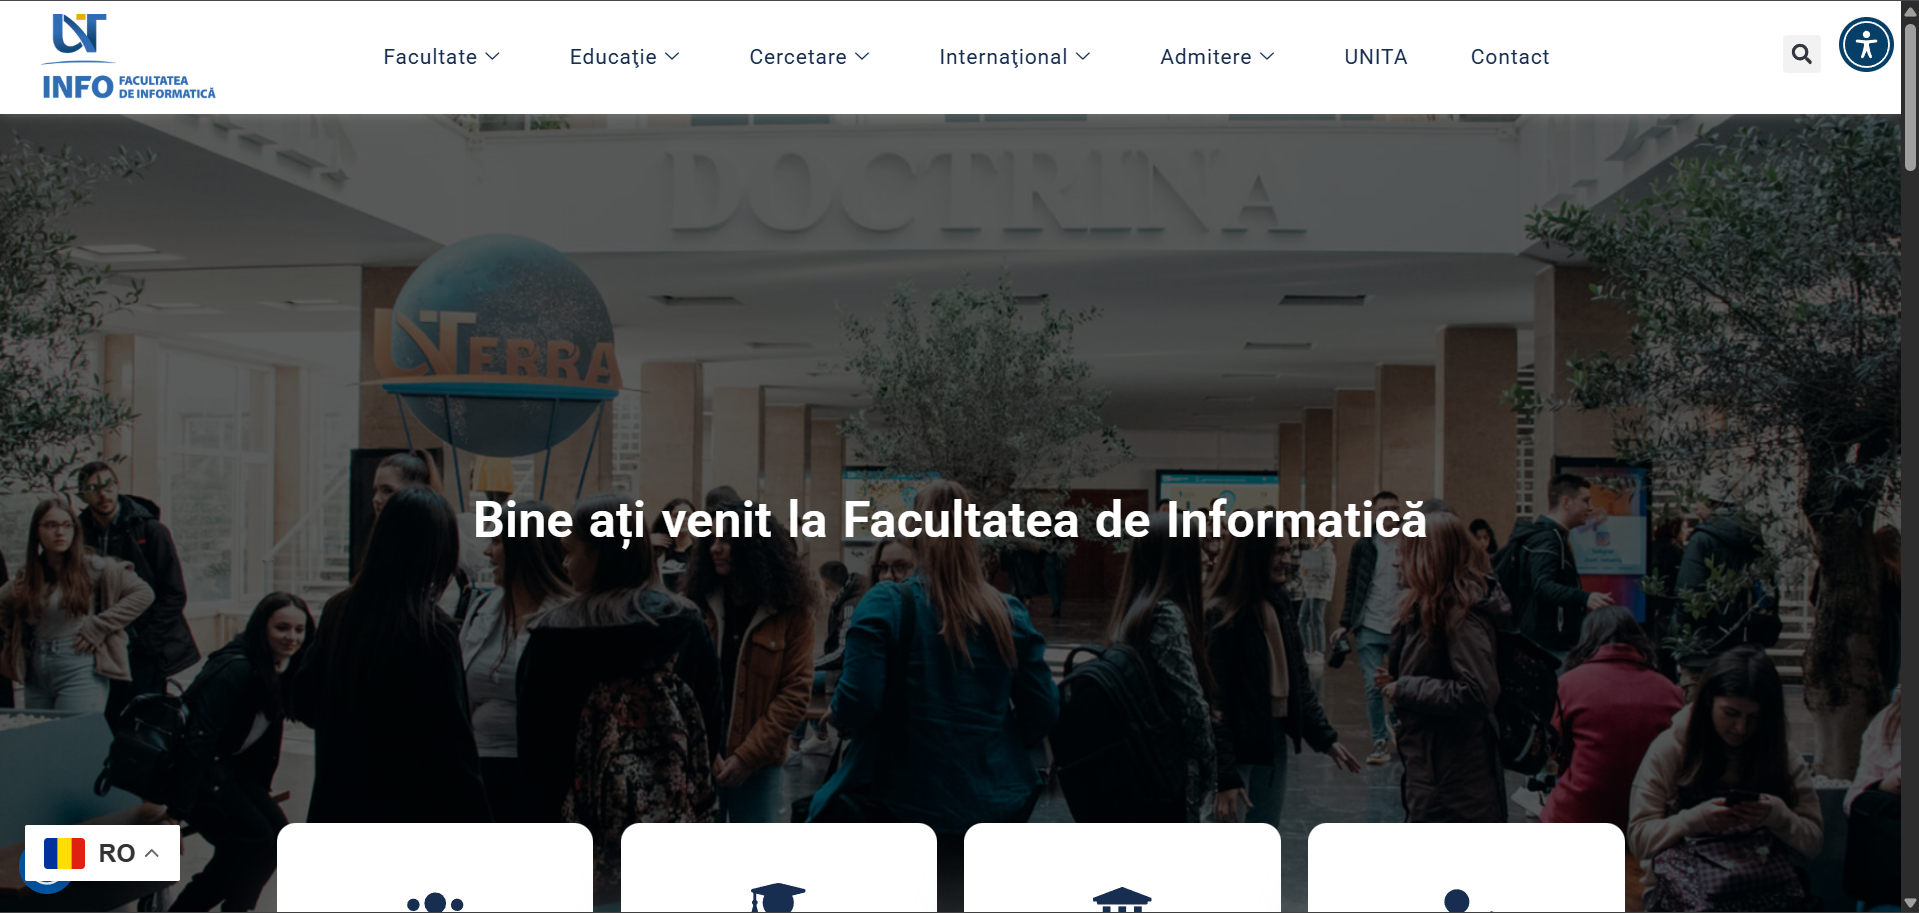
\includegraphics[width=15.4 cm]{imagini/site_uvt.png}
\caption{Site-ul Facultății}
\end{figure}

\section{Scopul și obiectivele proiectului}
\section{Structura lucrării}

% cap2
\chapter{Fundamente teoretice privind chatboții și extensiile browser}
\section{Noțiuni generale despre chatboți}
\section{Modele AI conversaționale și NLP}
\section{Arhitectura extensiilor Google Chrome}
\section{Sisteme de căutare și mapare a informațiilor}
\section{Tehnologii utilizate}

% cap3
\chapter{Proiectarea și arhitectura sistemului}
\section{Descriere generală a sistemului}
\section{Diagrama arhitecturală}
\section{Specificații pentru extensia Chrome}
\section{Proiectarea backend-ului și a API-ului}
\section{Modelul NLP și integrarea acestuia}
\section{Scenarii de utilizare}

% cap4
\chapter{Implementare}
\section{Implementarea extensiei Google Chrome}
\section{Implementarea backend-ului (API)}
\section{Integrarea modelului conversațional}
\section{Gestionarea interogărilor și generarea răspunsurilor}
\section{Probleme întâlnite și soluții}

% cap5
\chapter{Testare și evaluare}
\section{Metodologia testării}
\section{Testarea chatbotului}
\section{Rezultatele obținute}
\section{Analiza limitărilor}

% cap6
\chapter{Concluzii și direcții viitoare de dezvoltare}
\section{Concluzii asupra lucrării}
\section{Îmbunătățiri posibile}
\section{Direcții viitoare}

\chapter{Plan de activitate}

Realizarea lucrării de licență este organizată pe etape clare, distribuite astfel:


Decembrie: Documentare și analiză. Studierea conceptelor de bază privind chatboții, extensiile Google Chrome, arhitectura web a UVT, metode de procesare a limbajului natural și modele conversaționale.

Ianuarie: Proiectare arhitectură chatbot. Definirea componentelor: extensie Chrome, backend API, modul NLP, sistem de mapare a site-urilor UVT.

Februarie - Martie: Implementare extensie Chrome și backend. Dezvoltarea interfeței extensiei, conectarea la API, implementarea mecanismului de procesare a întrebărilor.

Aprilie: Integrare cu resursele UVT și testare. Validarea răspunsurilor chatbotului, testarea navigării asistate, optimizări ale modelului.

Mai: Finalizare lucrare și pregătire prezentare. Redactarea finală a lucrării, generarea anexelor, pregătirea prezentării pentru comisie.




\bibliographystyle{alpha}
\nocite{*}
\bibliography{mybib}
\addcontentsline{toc}{chapter}{Bibliography}

\end{document} 
